\documentclass[10pt]{article}\usepackage[]{graphicx}\usepackage[]{xcolor}
% maxwidth is the original width if it is less than linewidth
% otherwise use linewidth (to make sure the graphics do not exceed the margin)
\makeatletter
\def\maxwidth{ %
  \ifdim\Gin@nat@width>\linewidth
    \linewidth
  \else
    \Gin@nat@width
  \fi
}
\makeatother

\definecolor{fgcolor}{rgb}{0.345, 0.345, 0.345}
\newcommand{\hlnum}[1]{\textcolor[rgb]{0.686,0.059,0.569}{#1}}%
\newcommand{\hlstr}[1]{\textcolor[rgb]{0.192,0.494,0.8}{#1}}%
\newcommand{\hlcom}[1]{\textcolor[rgb]{0.678,0.584,0.686}{\textit{#1}}}%
\newcommand{\hlopt}[1]{\textcolor[rgb]{0,0,0}{#1}}%
\newcommand{\hlstd}[1]{\textcolor[rgb]{0.345,0.345,0.345}{#1}}%
\newcommand{\hlkwa}[1]{\textcolor[rgb]{0.161,0.373,0.58}{\textbf{#1}}}%
\newcommand{\hlkwb}[1]{\textcolor[rgb]{0.69,0.353,0.396}{#1}}%
\newcommand{\hlkwc}[1]{\textcolor[rgb]{0.333,0.667,0.333}{#1}}%
\newcommand{\hlkwd}[1]{\textcolor[rgb]{0.737,0.353,0.396}{\textbf{#1}}}%
\let\hlipl\hlkwb

\usepackage{framed}
\makeatletter
\newenvironment{kframe}{%
 \def\at@end@of@kframe{}%
 \ifinner\ifhmode%
  \def\at@end@of@kframe{\end{minipage}}%
  \begin{minipage}{\columnwidth}%
 \fi\fi%
 \def\FrameCommand##1{\hskip\@totalleftmargin \hskip-\fboxsep
 \colorbox{shadecolor}{##1}\hskip-\fboxsep
     % There is no \\@totalrightmargin, so:
     \hskip-\linewidth \hskip-\@totalleftmargin \hskip\columnwidth}%
 \MakeFramed {\advance\hsize-\width
   \@totalleftmargin\z@ \linewidth\hsize
   \@setminipage}}%
 {\par\unskip\endMakeFramed%
 \at@end@of@kframe}
\makeatother

\definecolor{shadecolor}{rgb}{.97, .97, .97}
\definecolor{messagecolor}{rgb}{0, 0, 0}
\definecolor{warningcolor}{rgb}{1, 0, 1}
\definecolor{errorcolor}{rgb}{1, 0, 0}
\newenvironment{knitrout}{}{} % an empty environment to be redefined in TeX

\usepackage{alltt}
\usepackage{color}
\usepackage[italian,english]{babel}
\usepackage[margin=2cm]{geometry}
\usepackage{bm}
\usepackage{tikz}
\usepackage[utf8x]{inputenc}
\usepackage{amsmath,amssymb}
\usepackage{apacite}
\usepackage[bottom]{footmisc} 


\usepackage{float}
\floatstyle{boxed}
\newfloat{program}{btp}{lop}
\floatname{program}{Box}
\usepackage{mdframed}
\definecolor{boxcol}{RGB}{213,226,238}
\newmdenv[linecolor=boxcol,backgroundcolor=boxcol]{comments}




\IfFileExists{upquote.sty}{\usepackage{upquote}}{}
\begin{document}

\title{Implementing significance testing for the Overlapping Index using Permutation Test}
\author{Ambra Perugini, Giulia Calignano, Massimo Nucci, Livio Finos, Massimiliano Pastore}

\maketitle



%\section{Introduction}

%%% It is also optimal when the assumptions of linear regression (i.g. normality, homoschedasticity etc.) are not met, as the index is calculated on the empirical distributions \cite{pastore2015analisi}. If we think about a t-test, which is a comparison of two groups on a given variable, it is a simple form of linear regression and therefore relies on the assumptions of the residuals. There are cases, such as reaction times, when said assumptions would be violated if not properly taken into account. There are cases in which you could even have same mean in two populations over a given variable, but the distributions differ in other parameters in a way that they are actually very different from each other (see figure \ref{fig:equalmeans}).

\section{Overlapping Index}

The overlapping index ($\eta$) is an intuitive way to define the area intesected by two or more probability density functions \cite{pastore2019measuring}. In a simple way, two distributions are similar when their distribution functions overlap, and as $\eta$ diminishes, the two distributions differ. The index $\eta$ of two empirical distributions varies from zero -- when the distributions are completely disjoint -- and one -- when they are completely overlapped \cite{pastore2018overlapping}. The simple interpretation of the overlapping index ($\eta$) makes its use particularly suitable for many applications \cite{moravec1988sensor, viola1997alignment, inman1989overlapping, milanovic2002decomposing}.

Assuming two probability density functions $f_A (x)$ and $f_B (x)$, the overlapping index $\eta: \mathbb{R}^n \times \mathbb{R}^n \to [0,1] $ is formally defined in the following way:


\begin{eqnarray}
\eta (A,B) = \int_{\mathbb{R}^n} min [f_A (x),f_B (x)] dx
\end{eqnarray} 

where, in the discrete case, the integer can be replaced by summation. As previously mentioned, $\eta (A,B)$ is normalized to one and when the distributions of A and B do not have points in common, meaning that $f_A (x)$ and $f_B (x)$ are disjoint, $\eta (A,B) = 0$. This index provides an intuitive way to quantify the agreement between $A$ and $B$ based on their density functions \cite{inman1989overlapping}. 






\vspace{.3cm}

In theory the two distributions are defined in the following way: 
$y_1 \sim \text{Normal}(10, 2)$ 
$y_2 \sim \text{Unif}(0, 20)$  

The true $\eta = 0.43$.


\vspace{.3cm}
To quickly illustrate a visual representation of the overlapping area in two given distributions we present the following example: a sample of 30 observations generated from a normal distribution with mean of 10 and standard deviation on 2 and a sample of 30 generated from a random uniform with the minimum value of 0 and the maximum of 20.





The figure \ref{fig:equalmeans} shows how two distributions with almost same mean could still be very different from each other with the overlapping area being $\hat{\eta} = 0.46$. 




\begin{knitrout}
\definecolor{shadecolor}{rgb}{0.969, 0.969, 0.969}\color{fgcolor}\begin{figure}

{\centering 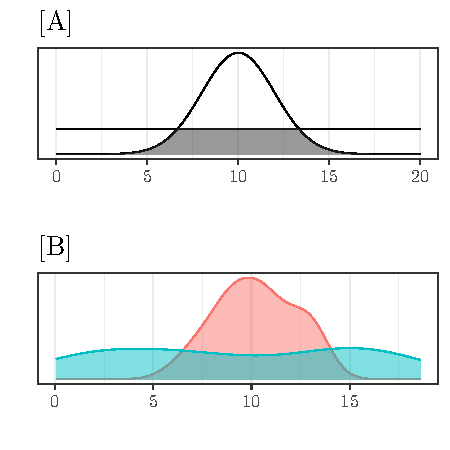
\includegraphics[width=\maxwidth]{figure/equalmeans-1} 

}

\caption[Comparison of a normal distribution and a uniform distribution with same mean]{Comparison of a normal distribution and a uniform distribution with same mean.}\label{fig:equalmeans}
\end{figure}

\end{knitrout}


In this case, a t-test would not be able to detect such difference, as it does not take into account the different variance in the two groups. Even when using a Welch test, which does not assume equal variance, the test does is less informative ($t = 0.881$, $p = 0.384$) compared to the overlapping index.

\subsection{Permutation approach}

 Now we will introduce another approach which does not rely on the assumptions of linear models: the permutation approach. This is a non-parametric statistical method that can be used to determine statistical significance and it is most useful when the assumptions of parametric tests are not met \cite{pesarin2010permutation}. What the test does is to rearrange the data in many different ways and recalculates the test statistic each time. If we are thinking about a simple mean comparison (a t-test), the data in the two groups are mixed over and over and the t-value is calculated each time. If the two groups come from the same population, mixing the labels should give similar results to the ones observed. Else, if the two groups come from different populations, mixing tags should lead to very different results. From the empirical density of the permuted values it is possible to calculate the p-value as the probability to obtain an equal or more extreme value compared to the observed one. 

\subsection{Application of permutation test to the overlapping index}

If we are reasoning from the perspective of Null Hypothesis Significance Testing (NHST), we should define the null hypothesis as follows: $H_0: \eta = 1$,  meaning there is no difference between the distributions of data in the population. For this reason, it is more intuitive to work with the complement of $\eta$, which is  $1-\eta = \zeta$ which is the area of non-overlap, therefore, defining the null hypothesis as  $H_0:\zeta = 0$. When testing the difference between the two distributions, we will no longer be working with $\eta$, but with the complement $\zeta$. 

Even though the overlapping index has a simple interpretation, one could argue that it does not provide information on the significance of the parameter $\eta$, therefore, we decided to implement permutation testing to offer to the ones interested a value of significance. In particular, we implemented permutations test, to give a tool that tests differences in distributions in cases where other tests' assumptions would be violated.

The algorithm estimates the value of $\zeta$ on the observed data ($\hat{\zeta}$). Then, through permutation, the values of the two groups are randomly re-assigned to the groups for B times, estimating again the new value of  $\hat{\zeta}_b$. The times in which the estimate of $\hat{\zeta}_b$ on permuted data is higher than the one observed on real data is estimated ($\hat{\zeta}_b > \hat{\zeta}$) and then the found value is divided by B, returning the $p$-value. This approach is equivalent to the traditional parametric tests.

A typical example of data not respecting previously said assumptions is reaction times and for this purpose we present a real case of a dataset available online (citation of the OSF repository) on reaction times of word reading of high and low frequency words in English and we implement on the overlapping function the permutation test. 










\begin{knitrout}
\definecolor{shadecolor}{rgb}{0.969, 0.969, 0.969}\color{fgcolor}\begin{figure}

{\centering 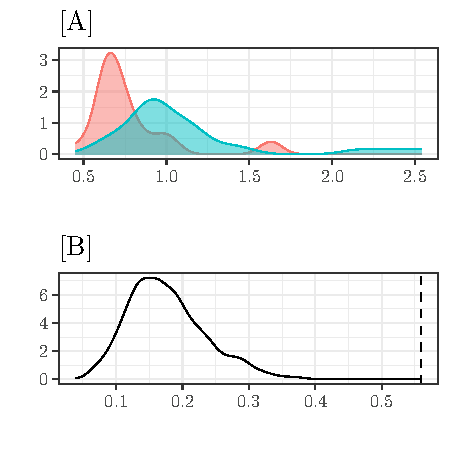
\includegraphics[width=\maxwidth]{figure/ex2-1} 

}

\caption{$\hat{\zeta} = 0.56$. [A] Distribution of reaction times of word reading of high and low frequency words in English; [B] Distribution of $\hat{\zeta}$ obtained with 2000 permutations of the data.}\label{fig:ex2}
\end{figure}

\end{knitrout}
In the figure \ref{fig:ex2}[A] are represented the densities of reaction times of word reading of high and low frequency words in English; the obtained value of $\hat{\zeta}$ is 0.56. In figure \ref{fig:ex2}[B] is represented the distribution of the values of $\hat{\zeta}$ obtained with 2000 permutations; let us calculate the $p$-\emph{value}:

\begin{knitrout}
\definecolor{shadecolor}{rgb}{0.969, 0.969, 0.969}\color{fgcolor}\begin{kframe}
\begin{alltt}
\hlkwd{sum}\hlstd{( zperm} \hlopt{>} \hlstd{obsz )} \hlopt{/} \hlkwd{length}\hlstd{( zperm )}
\end{alltt}
\begin{verbatim}
[1] 0
\end{verbatim}
\end{kframe}
\end{knitrout}

The difference is statistically significant and the $t$ test:
\begin{knitrout}
\definecolor{shadecolor}{rgb}{0.969, 0.969, 0.969}\color{fgcolor}\begin{kframe}
\begin{verbatim}
> with( xList, t.test( x1, x2 ) ) 
 
	Welch Two Sample t-test 
 
data:  x1 and x2 
t = -3, df = 46, p-value = 0.002 
\end{verbatim}
\end{kframe}
\end{knitrout}


\section{Simulation study}

To evaluate the performance of the permutation test applied to the overlapping index, we performed a simulation study. The aim is to generate data for a set of scenarios distinguishing mean, variance and shape of the populations and compare the $\zeta$ perm test to other commonly used tests in terms of type I error control and power. 

\subsection{Data generation}

In the simulation, two density distributions will be compared for many different scenarios. The first distribution will always be a normal standard distribution with $\mu = 0$ and $\sigma = 1$. 
To simulate data for the second distribution we use the Skew-Normal distribution \cite{azzalini:1985}, which is defined in the following way: given $\xi \in \mathbb{R}$, $\omega \in \mathbb{R}^{+}$ and $\alpha \in \mathbb{R}$, then for $y \in \mathbb{R}$ we have  
\begin{eqnarray}
\mathcal{SN}(y|\xi, \omega, \alpha) = \frac{1}{\omega \sqrt{2\pi}} exp \left[ -\frac{1}{2} \left( \frac{y-\xi}{\omega} \right)^2  \right] \left[ 1+ \text{erf}\left( \alpha \left( \frac{y-\xi}{\omega\sqrt{2}}\right) \right) \right]
\end{eqnarray} 
in which $$\text{erf}(z) = \frac{2}{\sqrt{\pi}} \int_{0}^{z} e^{-t^2} dt $$ is the \emph{error function}.
When $\xi = 0$, $\omega = 1$ and $\alpha = 0$ the distribution is a standard normal distribution.

The parameter $\alpha$ determines the symmetry, $\xi$ is the mean value and $\omega$ determines the variance. Therefore, this distribution is suitable to generate data modelling both the distance between means (the effect size), symmetry and variance.

Mean and variance of the Skew-Normal are respectively: 
\begin{eqnarray}\label{eq:musigmaSN}
\begin{array}{l}
\mu = \xi + \omega \delta \sqrt{2/\pi} \\
\sigma^2 = \omega^2 [1- (2\delta^2)/\pi]
\end{array}
\end{eqnarray}
in which $\delta = \alpha / \sqrt{1 + \alpha^2}$. Based on the equations (\ref{eq:musigmaSN}) we can determine the values to assign to the parameters $\xi$ e $\omega$ in function of $\mu$ and $\sigma$ with the equations:

\begin{eqnarray}\label{eq:xiomegaSN}
\begin{array}{l}
 \xi = \mu - \omega \delta \sqrt{2/\pi} \\
 \omega = \sqrt{\sigma^2/ [1- (2\delta^2)/\pi]}
\end{array}
\end{eqnarray}

The Skwe-Normal distribution is optimal for our purpose as it allows to have control over parameters of skewness and kurtosis, as shown in figure \ref{fig:scenari}.

\begin{knitrout}
\definecolor{shadecolor}{rgb}{0.969, 0.969, 0.969}\color{fgcolor}\begin{figure}

{\centering 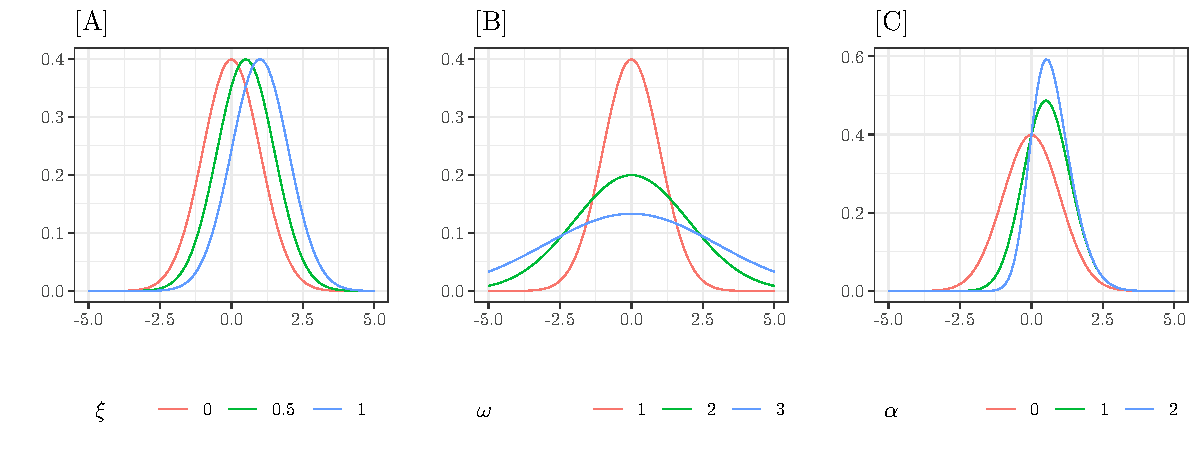
\includegraphics[width=\maxwidth]{figure/scenari-1} 

}

\caption[Skew-Normal distribution ($\xi$,$\omega$,$\alpha$)]{Skew-Normal distribution ($\xi$,$\omega$,$\alpha$); [A] the parameter $\xi$ controls the mean, [B] the parameter $\omega$ the variance and [C] the parameter  $\alpha$ the simmetry.}\label{fig:scenari}
\end{figure}

\end{knitrout}


\subsection{Simulation design}





In the simulation we confront two samples extracted from a Skew-Normal, the first one is generated from $\mathcal{SN}(0,1,0)$, which is the Standard-Normal distribution, and the second one from $\mathcal{SN}(\xi,\omega,\alpha)$ where parameters are chosen each time based on the experimental design as follows:


\begin{itemize}

  \item $n = (10, 20, 50, 100, 500)$; sample size, equal in the two samples;
  \item $\delta = (0, 0.2, 0.5, 0.8)$; mean of the second sample, which corresponds also to the difference between the two groups, the first one has always $\mu = 0$;
  \item $\sigma = (1, 2, 3)$; standard deviation of the second sample;
  \item $\alpha = (0, 2, 10)$; degree of asymmetry (skewness) of the second sample. 
  \item N simulation: 1000 for each combination of parameters

\end{itemize}


For each of the $5 \times 4 \times 3 \times 3 = 180$ conditions we generated 1000 sets of data on which we performed the analysis.

In figure \ref{fig:alpha0} are graphically represented the 36 scenarios of data generation, the black curves are the first sample, always a $\mathcal{SN}(0,1,0)$, and the red curves are relative to the second sample $\mathcal{SN}(\xi,\omega,\alpha)$.

For each combination $n \times \delta \times \sigma \times \alpha$, on the generated data were performed the following tests: 
\begin{itemize}
 \item $t$ test for independent samples, assuming equal variance
 \item Welch test for independent samples 
 \item Wilcoxon test for independent samples
 \item Permutation test on the complement of the overlapping index, $\zeta = 1-\eta$, which therefore becomes an index of difference between groups
 \item $F$ test of omogeneity of variances
 \item Kolmogorov-Smirnov test for confronting two distributions
\end{itemize}

% \begin{itemize}
%  \item T-test: a parametric test used to test if the mean value of a distribution is significantly different from the one of another group;
%  \item Welch test: as a variation of the independent sample t-test, this one does not assume equal variance between the two groups, and is therefore more robust when variance or sample size is different in the two groups;
%  \item Wilcoxon Signed-Rank Test: is a non parametric test to compare two related samples or a single repeated measure on the same sample when the data is not normally distributed and is based on the mean rank difference;
%  \item Variance test (F-test): a parametric test to compare the variance in two groups or more. It relies on normality assumptions and the null hypotesis is equal variance in the two groups;
%  \item Kolmogorov-Smirnov Test: a non-parametric test used to either compare a sample distribution to a known distribution or to compare two samples to test if they come from the same unknown distribution;
%  \item T-test with permutation approach: is a test on means but the p-value is calculated through permutations, therefore it is not parametric;
%  \item F-test with permutation approach: is a test on variance and again, it is a non parametric test calculating the p-value through permutations of the data;
%  \item Overlapping index $\zeta$ with permutation approach.
% \end{itemize}

\begin{knitrout}
\definecolor{shadecolor}{rgb}{0.969, 0.969, 0.969}\color{fgcolor}\begin{figure}

{\centering 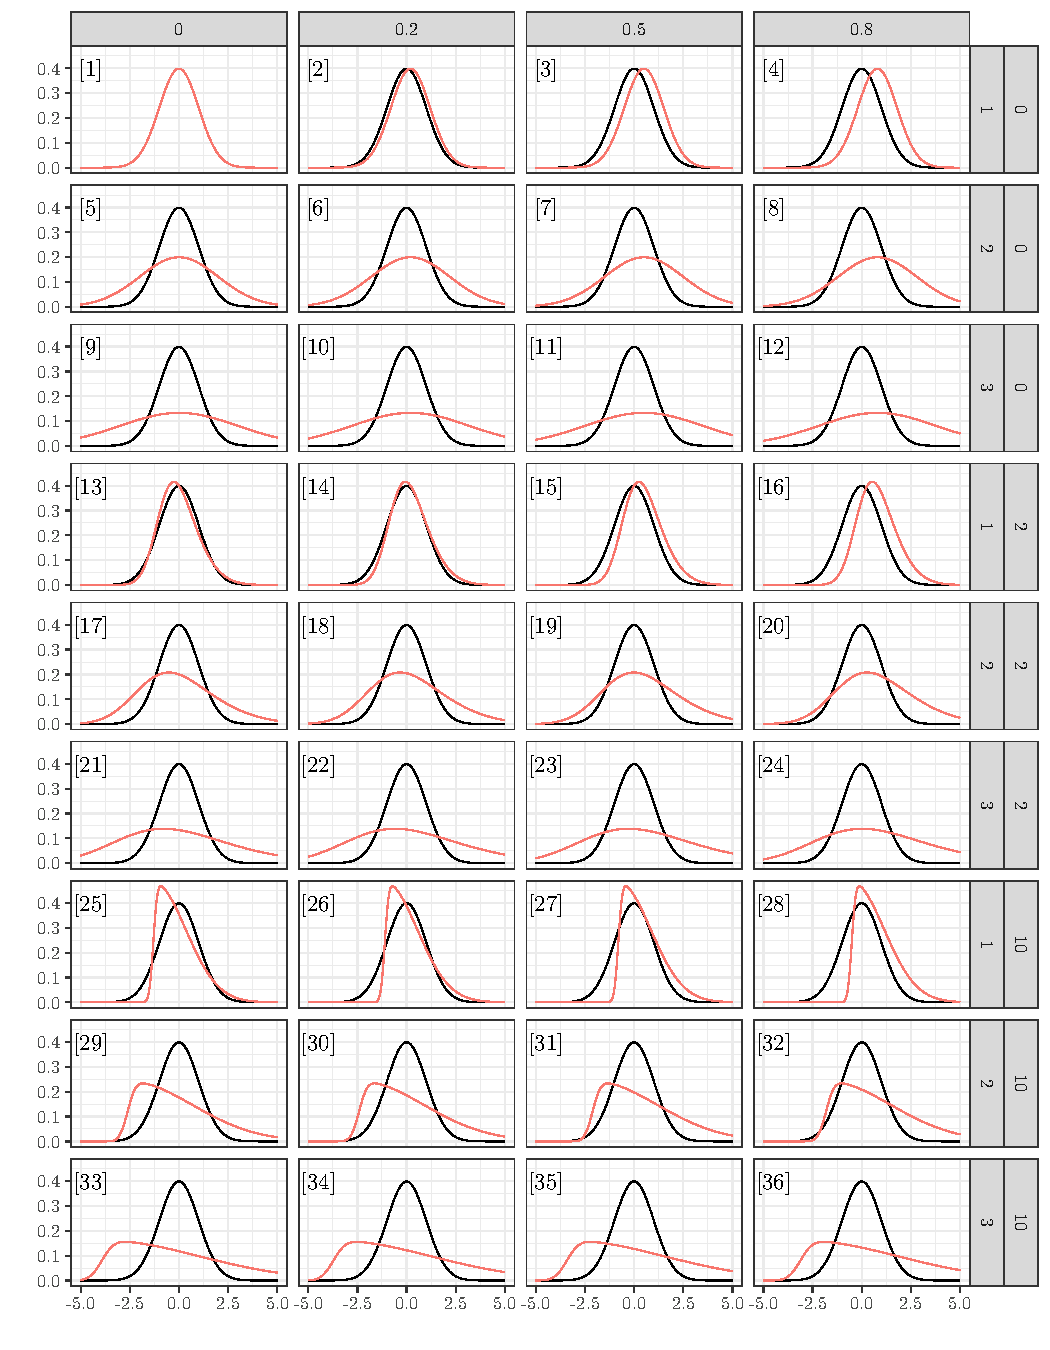
\includegraphics[width=\maxwidth]{figure/alpha0-1} 

}

\caption[ Generative data distributions in function of $\delta$ (column panels) and $\sigma$ (row panels)]{ Generative data distributions in function of $\delta$ (column panels) and $\sigma$ (row panels). The black curves are the first sample, $\mathcal{SN}(0,1,0)$, the red ones represent second sample.}\label{fig:alpha0}
\end{figure}

\end{knitrout}

\subsection{Definition of Null Hypothesis}

Each test relies on different assumptions and tests a specific null hypothesis. 

\subsubsection{$t$ test}


This is the classic case of a test for independent samples assuming equal variances:
 
\begin{eqnarray*}
H_0: \mu_1 - \mu_2 = 0 \mbox{ con } \sigma_1 = \sigma_2
\end{eqnarray*}

Therefore, in the scenarios from which the samples come from populations with same mean $\mathcal{SN}(0,\sigma,\alpha)$ -- figure \ref{fig:alpha0}, panels in the first left column -- type I error control is estimated, meanwhile, power is estimated for the other scenarios.

\subsubsection{Welch test}

This is the $t$ test modified when homogeneity of variances is not respected:

\begin{eqnarray*}
H_0: \mu_1 - \mu_2 = 0 \mbox{ con } \sigma_1 \neq \sigma_2
\end{eqnarray*}

Control of type I error is estimated for the same scenarios as for the $t$ test, as well as for the power.

\subsubsection{Wicoxon-Mann-Whitney test}

This is the test on ranks which assumes
 
\begin{eqnarray*}
H_0: P(X_1 > X_2) = P(X_2 > X_1) = 0.5
\end{eqnarray*} 

in which $X_1$ and $X_2$ are the random variables representing the observations extracted from the two populations. In this case, the only scenario in which $H_0$ is true is in panel [1].

\subsubsection{$\zeta$ permutation test}

Since $\zeta = 1 - \eta$, in which $\eta$ is the area of overlapping of the empirical distributions, the null hypothesis of the test is $$H_0: \zeta = 0$$ which implies that the data comes from the same population, or from populations with same shape (mean, variance and skewness). Therefore, the only condition in which $H_0$ is true is the first panel. 

\subsubsection{$F$ test}

This is the test of homogeneity of variances $$H_0: \sigma^2_1 = \sigma^2_2$$ the condition is true in all scenarios where $(\delta,1)$, panels [1:4, 13:16, 25:28]. In those scenarios we estimate type I error, in all the others we calculate power.

\subsubsection{Kolmogorov-Smirnov test}

This test compares the cumulative distributions $$H_0: F(X_1) = F(X_2)$$ therefore, the null hypothesis should be true in panel [1], as it is for the $\zeta$ permutation test.

Taking into account those null hypothesis and assumptions, we will compute type I error by counting how many times the test is significant when the null is true, and the power by counting how many times it will be significant when $H_0$ is not true. Then we will consider separately the cases in which assumptions are respected and when they are not.

\section{Results}

Figure \ref{fig:correlazioni} represents the correlation matrix between the indexes in all experimental conditions, calculated on 180000 indexes obtained from the simulation. two subgroups are clearly visible: the first group with tests on mean and ranks, and the second one on tests about the shape, the $F$ test is not correlated with the others. 



\begin{knitrout}
\definecolor{shadecolor}{rgb}{0.969, 0.969, 0.969}\color{fgcolor}\begin{figure}[!h]

{\centering 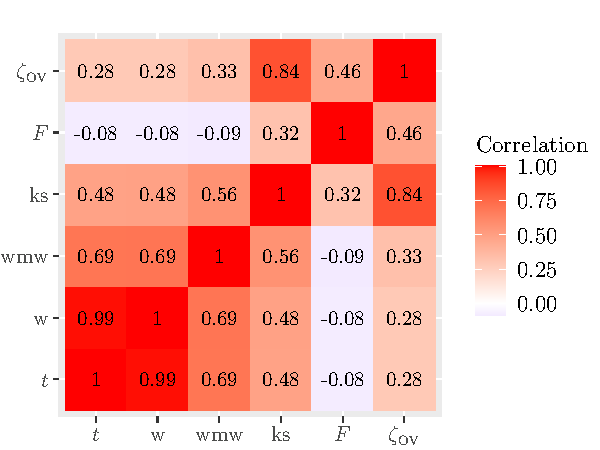
\includegraphics[width=\maxwidth]{figure/correlazioni-1} 

}

\caption[Correlation matrix among $p$-values $(N = 180000)$]{Correlation matrix among $p$-values $(N = 180000)$.}\label{fig:correlazioni}
\end{figure}

\end{knitrout}

\subsection{Global type I error and power}





In figure \ref{fig:global}, is represented type I error in panel A and power in panel B, for all scenarios it is evaluated when $H_0$ is either true or false, as different tests have different null hypothesis. Panel A shows how they all control well enough for type I error, except for the $F$ test. The $\zeta$ perm test outperforms all other tests in terms of power, already from small sample sizes, once more, the $F$ test is the exception, as it is a test on variance.

\begin{knitrout}
\definecolor{shadecolor}{rgb}{0.969, 0.969, 0.969}\color{fgcolor}\begin{figure}

{\centering 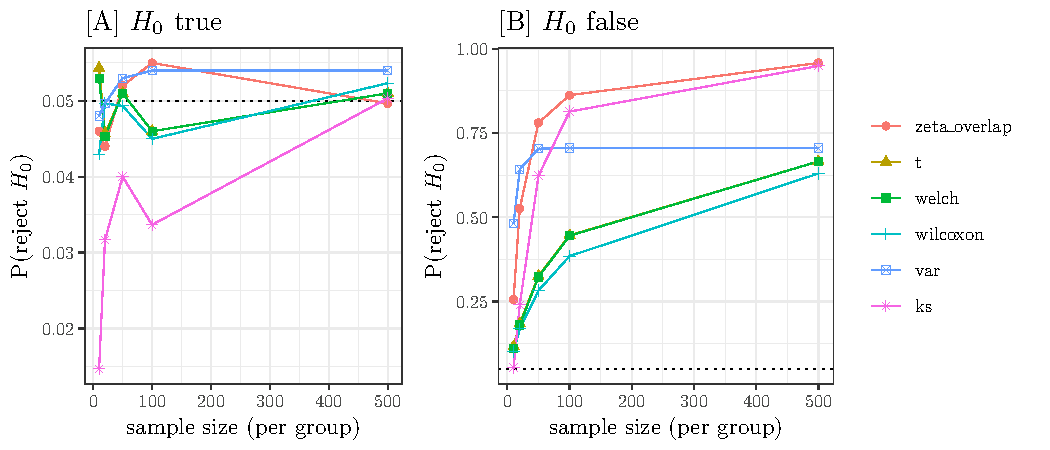
\includegraphics[width=\maxwidth]{figure/global-1} 

}

\caption[l]{Control of type I error [A] and power [B] in various tests taking into account for each of them in which scenario $H_0$ is true or false.}\label{fig:global}
\end{figure}

\end{knitrout}

\subsection{Assumptions and type I error and power}

In the top row of figure \ref{fig:assunzioni} are represented type I error and power for cases in which assumptions are respected. The patter is similar to the scenario in \ref{fig:global} where there was no distinction for the assumptions, confirming the good control of type I error of the $\zeta$ perm test and greater power of the test in comparison to the others.
As not all tests that we performed imply assumptions, we only computed type I error and power for those tests that can have the assumptions violated ($t$ test, $F$ test, Welch test). What emerges is a bad control of type I error of the $F$ test.




\begin{knitrout}
\definecolor{shadecolor}{rgb}{0.969, 0.969, 0.969}\color{fgcolor}\begin{figure}

{\centering 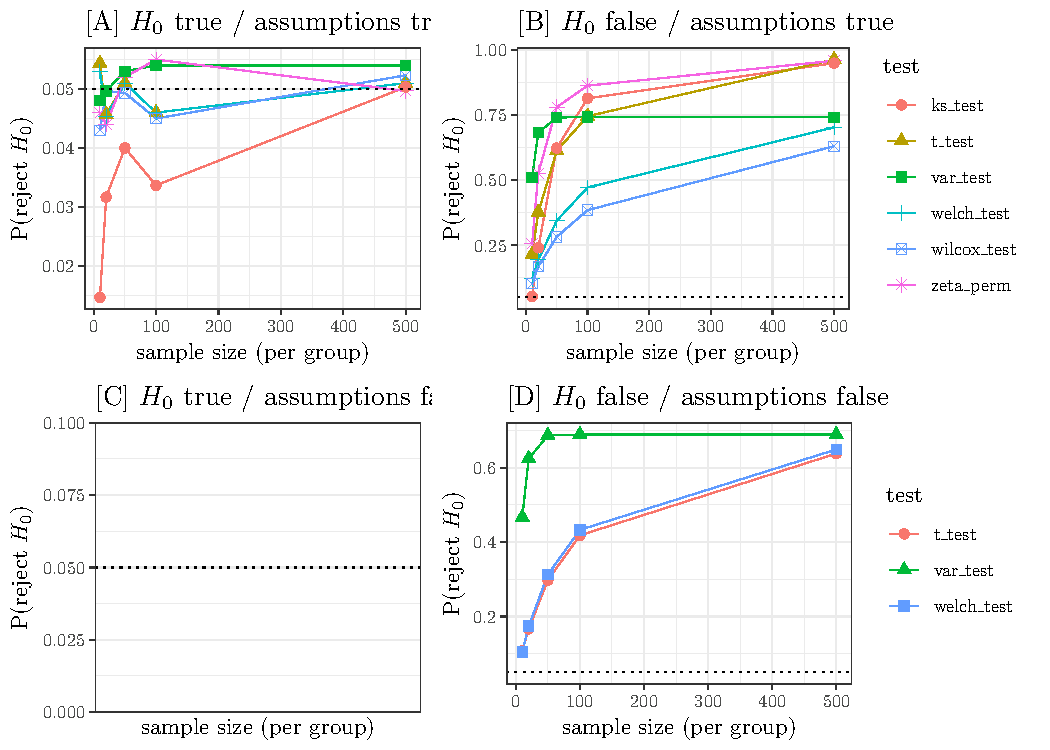
\includegraphics[width=\maxwidth]{figure/assunzioni-1} 

}

\caption[Control of type I error and power for scenarios in which assumptions are respected (top panels) and when they are not (bottom panels)]{Control of type I error and power for scenarios in which assumptions are respected (top panels) and when they are not (bottom panels).}\label{fig:assunzioni}
\end{figure}

\end{knitrout}



%%\subsection{gara tra $\zeta$ perm da solo e t-test, ks e var test }

\section{Discussion}

\newpage

\section{Legenda}

$\eta$ is the area of overlap

$\zeta$ is the area of non overlap, therefore $1 - \eta$

$\mu$ is the parameter of the mean of the normal standard 

$\sigma$ is the standard deviation of the normal standard

$\alpha$ determins the simmetry of the skew-normal

$\xi$ is the mean value of the skew-normal

$\omega$ determines the variance of the skew-normal

$\delta$ is the difference between the two means



\newpage
\bibliographystyle{apacite}
\bibliography{overlap}




\end{document}







\end{document}



\end{document}
